\documentclass[10pt]{beamer}

\usepackage{listings}
\usepackage{tikz}
\DeclareMathOperator{\Ima}{Im}
\usetikzlibrary{automata,positioning}
\usepackage{graphicx}

\usecolortheme{seagull}
\useoutertheme{infolines}
\usefonttheme[onlymath]{serif}

\title{Creating a Robust AspectMATLAB Compiler}
\author{Hongji Chen \and Laurie Hendren (advisor)}
\date[September 1, 2016]{UCORE'16}

\begin{document}

\frame{\maketitle}

\begin{frame}
\frametitle{Aspect oriented programming}
\begin{itemize}
    \item Pointcut $\Rightarrow$ pattern
    \item Pointcut advice $\Rightarrow$ action
\end{itemize}
\end{frame}

\begin{frame}[fragile]
\frametitle{Generating Dynamic Call Graph Using AspectMATLAB}
\framesubtitle{A quick guide to AspectMATLAB}
\begin{itemize}
\item <1-> Pointcuts(patterns)
\begin{lstlisting}[basicstyle=\small, language=MATLAB]
patternCall : call(*(..))
patternExecution : execution(*(..))
\end{lstlisting}
\item <2-> Pointcut advices(actions)
\begin{lstlisting}[basicstyle=\small, language=MATLAB]
actionCallBefore : before call(*(..)) : (name)
  disp(sprintf('entering %s', name));
end
actionExecution : around execution(*(..)) : (name)
  ticHandle = tic;
  proceed();
  elapsedTime = toc(ticHandle);
  disp(sprintf('executed %s, Elapsed time: %d', name, elapsedTime));
end
actionCallAfter : after call(*(..)) : (name)
  disp(sprintf('returning from %s', name));
end
\end{lstlisting}
\end{itemize}

\end{frame}

\begin{frame}[fragile]
\frametitle{Generating Dynamic Call Graph Using AspectMATLAB}
\framesubtitle{A quick guide to AspectMATLAB}
\begin{columns}
\begin{column}[T]{0.5\textwidth}
\begin{lstlisting}[basicstyle=\small, language=MATLAB]
function [] = launchingFunc()
  % join point here 
  % entrance point
  foo();    % join point here
end

function [] = foo()
  % join point here
  goo();    % join point here
  % do something here
  goo();    % join point here
end

function [] = goo()
  % join point here
  % do something here
end
\end{lstlisting}    
\end{column}

\pause

\begin{column}[T]{0.5\textwidth}
\textbf{Executing Result}
\begin{lstlisting}[basicstyle=\small]
entering foo
entering goo
executed goo, Elapsed time: <double>
returning from goo
entering goo
executed goo, Elapsed time: <double>
returning from goo
executed foo, Elapsed time: <double>
returning from foo
executed launchingFunc, Elapsed time: <double>
\end{lstlisting}
\end{column}
\end{columns}
\end{frame}

\begin{frame}
\frametitle{Previous Work}
\begin{itemize}
    \item Toheed Aslam's AspectMATLAB Compiler
    \item Andrew Bodzay's AspcetMATLAB++ Compiler
    \item McSAF Framework, and Kind Analysis
    \item Samuel Suffos's Parser
\end{itemize}
\end{frame}

\begin{frame}
\frametitle{Improvement and Contributions}
\begin{itemize}
    \item Use of More Robust Front-end
    \item Clear Grammar
    \item Semantic Validation
    \item More Robust Transforming Strategy
    \item Extended Argument Matching
\end{itemize}
\end{frame}

\begin{frame}
\frametitle{Compiler Structure}
\textbf{Existing AspectMATLAB Compiler Structure}
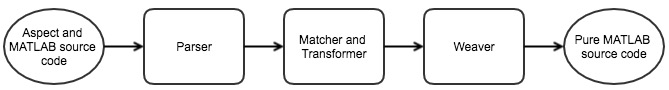
\includegraphics[scale=0.4]{old_structure}

\textbf{New AspectMATLAB Compiler Structure}
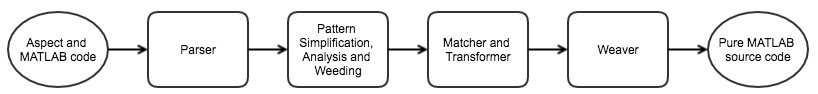
\includegraphics[scale=0.4]{new_structure}
\end{frame}

\begin{frame}[fragile]
\frametitle{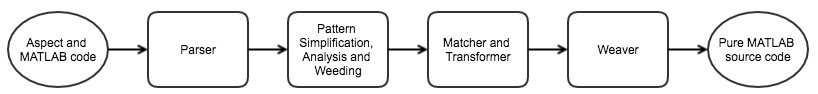
\includegraphics[scale=0.4]{new_structure}\\Parser}
\begin{itemize}
\item New parser built using ANTLR3
\item Extend set/get/call pattern to make patterns more clear
\begin{lstlisting}[basicstyle=\small, language=MATLAB]
get(x) & dimension([1, 1]) & istype(logical)    
\end{lstlisting}    
$\Rightarrow$
\begin{lstlisting}[basicstyle=\small, language=MATLAB]
get(x : [1,1]logical)    
\end{lstlisting}
\item allow dots wildcard to appear any where in the signature list
\begin{lstlisting}[basicstyle=\small, language=MATLAB]
dimension([1, .., 3])
\end{lstlisting}
\end{itemize}
\end{frame}

\begin{frame}
\frametitle{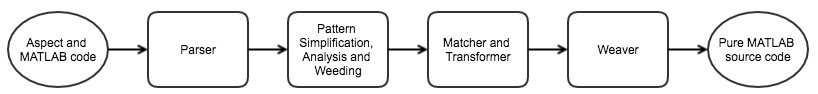
\includegraphics[scale=0.4]{new_structure}\\Semantic Validation} 
\begin{itemize}
    \item Basic Pattern classification
        \begin{itemize}
        \item Primitive pattern
        \item Modifier pattern
        \end{itemize}
    \item Pattern type analysis for compound pattern
    \item using logical equivalence to associate modifier pattern to  
          primitive pattern
    \item inspect primitive pattern individually.
\end{itemize}
\end{frame}

\begin{frame}[fragile]
\frametitle{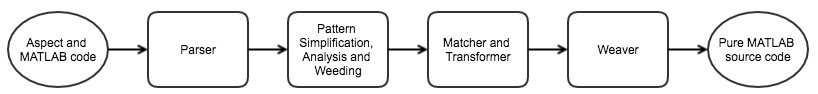
\includegraphics[scale=0.4]{new_structure}\\Semantic Validation} 
\framesubtitle{Examples}
matching under "before" case
\begin{lstlisting}[basicstyle=\small, language=MATLAB]
(get(x) | call(foo(..))) & ~(istype(logical) | dimension([1,1]))    
\end{lstlisting}
$\Rightarrow$
\begin{lstlisting}[basicstyle=\small, language=MATLAB]
(get(x) | call(foo(..))) & (~istype(logcial) & ~dimension([1,1]))    
\end{lstlisting}
$\Rightarrow$
\begin{lstlisting}[basicstyle=\small, language=MATLAB]
(get(x) & (~istype(logcial) & ~dimension([1,1]))) | 
    (call(foo(..)) & (~istype(logcial) & ~dimension([1,1])))
\end{lstlisting}
$\Rightarrow$                                                             \\
\textbf{Reject}
\end{frame}

\begin{frame}[fragile]
\frametitle{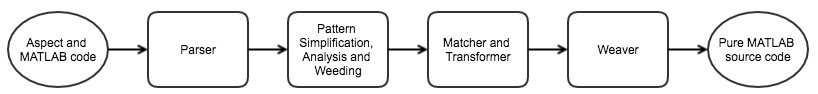
\includegraphics[scale=0.4]{new_structure}\\Matcher and
            Transformer}
\begin{itemize}
\item handling spanned comma separated list, e.g.
\begin{lstlisting}[basicstyle=\small, language=MATLAB]
c{:}    m(:).f    c{1:5}    
\end{lstlisting}
\item correctly resolve end expression
\begin{lstlisting}[basicstyle=\small, language=MATLAB]
m(1, end - 1)
\end{lstlisting}
\item better variable capture for set pattern
\begin{lstlisting}[basicstyle=\small, language=MATLAB]
[var1, var2] = foo();    
\end{lstlisting}
\item ...
\end{itemize}   
\end{frame}

\begin{frame}[fragile]
\frametitle{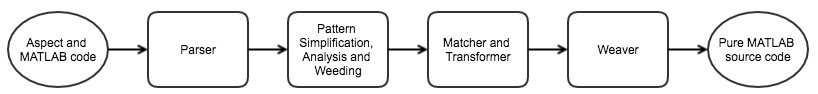
\includegraphics[scale=0.4]{new_structure}\\Weaver}
\framesubtitle{Extended Argument Signature List Matching}
\textbf{Current AspectMATLAB Compiler}
\begin{itemize}
    \item subroutine name
    \item number of subroutine input arguments
\end{itemize}
\begin{lstlisting}[basicstyle=\small, language=MATLAB]
call(foo(*,*,..))    
\end{lstlisting}

\textbf{New AspectMATLAB Compiler}
\begin{itemize}
    \item shape information of the argument
    \item type information of the argument
    \item subroutine outputs
\end{itemize}
\begin{lstlisting}[basicstyle=\small, language=MATLAB]
call(foo([1,1]logical, .., [3,..,3]integer) : [..]double)    
\end{lstlisting}
\end{frame}

\begin{frame}
\frametitle{Extended Argument Matching}
\begin{itemize}
    \item Collect Alphabet
    \item Building nondeterministic finite automaton for shape patterns
    \item Convert nondeterministic finite automaton into deterministic
          finite automaton
    \item Emit matcher function
\end{itemize}
\end{frame}

\begin{frame}[fragile]
\frametitle{Extended Argument Matching}
\framesubtitle{Collect Alphabet}
\textbf{Why?} We need a finite alphabet to built NFA and DFA. But, in MATLAB,
any valid identifier can be a valid type name, and dimension can be a list of
any positive integers.

Trivial solution. $\times$

\pause

Construct alphabet $\Sigma$ as follow:
\begin{itemize}
    \item $\epsilon \in \Sigma$
    \item if symbol $s$ appears in signature, then $s \in \Sigma$
    \item let $\sigma$ be a special symbol, denoting any other symbol that
          don't appear in the signature
\end{itemize}
Then the alphabet $\Sigma$ is a finite set, as we have a finite signature.

\pause
\begin{lstlisting}[basicstyle=\small, language=MATLAB]
call(foo(*, .., [1,*,..,2,3]double) : [..]logical, [2,2]*)
\end{lstlisting}
$\Sigma_{shape} = \lbrace \epsilon_{shape}, 1, 2, 3, \sigma_{shape} \rbrace$ \\
$\Sigma_{type} = \lbrace \epsilon_{type}, \text{double},
                         \text{logical}, \sigma_{type} \rbrace$              
\end{frame}

\begin{frame}[fragile]
\frametitle{Extended Argument Matching}
\framesubtitle{Building nondeterministic finite automaton for shape patterns}
\textbf{Pattern with only shape matching}
\begin{lstlisting}[basicstyle=\small, language=MATLAB]
dimension([1, *, .., 2, 3])
\end{lstlisting}
Alphabet : $\Sigma_{shape} = \lbrace \epsilon, 1, 2, 3, \sigma \rbrace$
\begin{tikzpicture}[shorten >=1pt,node distance=1.3cm,on grid,auto] 
    \node[state, initial]   (0)               {$0$};
    \node[state]            (1) [right of=0]  {$1$};
    \node[state]            (2) [right of=1]  {$2$};
    \node[state]            (3) [right of=2]  {$3$};
    \node[state]            (4) [right of=3]  {$4$};
    \node[state]            (5) [right of=4]  {$5$};
    \node[state]            (6) [right of=5]  {$6$};
    \node[state, accepting] (7) [right of=6]  {$7$};
    \path[->]
    (0)      edge node                 {$1$}                      (1)
    (1)      edge [bend left]node      {$1,2,3,\sigma$}           (2)
    (2)      edge node                 {$\epsilon$}               (3)
    (3)      edge [bend left]node      {$1,2,3,\sigma,\epsilon$}  (4)
    (4)      edge node                 {$\epsilon$}               (5)
    (5)      edge node                 {$2$}                      (6)
             edge [bend left]node      {$\epsilon$}               (2)
    (6)      edge node                 {$3$}                      (7);
\end{tikzpicture}
\textbf{Pattern with only type matching}
\begin{lstlisting}[basicstyle=\small, language=MATLAB]
call(foo(logical, *, .., double))
\end{lstlisting}
Alphabet : $\Sigma_{type} = \lbrace \epsilon, \text{logical}, 
                                    \text{double}, \sigma \rbrace$

\begin{tikzpicture}[shorten >=1pt,node distance=1.5cm,on grid,auto] 
    \node[state, initial]   (0)               {$0$};
    \node[state]            (1) [right of=0]  {$1$};
    \node[state]            (2) [right of=1]  {$2$};
    \node[state]            (3) [right of=2]  {$3$};
    \node[state]            (4) [right of=3]  {$4$};
    \node[state]            (5) [right of=4]  {$5$};
    \node[state, accepting] (6) [right of=5]  {$6$};
    \path[->] 
    (0)     edge [bend left]node     {$\text{logical}$}                    (1)
    (1)     edge [bend left]node     {$\Sigma_{type} \setminus \lbrace
                                       \epsilon \rbrace$}                  (2)
    (2)     edge node                {$\epsilon$}                          (3)
    (3)     edge node                {$\Sigma_{type}$}                     (4)
    (4)     edge node                {$\epsilon$}                          (5)
    (5)     edge [bend left]node     {$\text{double}$}                     (6)
            edge [bend left]node     {$\epsilon$}                          (2);
\end{tikzpicture}
\end{frame}

\begin{frame}[fragile]
\frametitle{Extended Argument Matching}
\framesubtitle{Convert NFAs into DFAs}
\textbf{Using subset construction method}

\begin{columns}
\begin{column}[T]{0.5\textwidth}
\begin{lstlisting}[basicstyle=\small, language=MATLAB]
dimension([1, *, .., 2, 3])
\end{lstlisting}
Alphabet Map : $\lbrace 1 = 1, 2 = 2, 3 = 3, \sigma = 4 \rbrace$             \\
Matrix representation of DFA in MATLAB:
\begin{lstlisting}[basicstyle=\small, language=MATLAB]
AM_FUNC_8 = [2, 6, 6, 6; 
             3, 3, 3, 3; 
             3, 4, 3, 3; 
             3, 4, 5, 3; 
             3, 4, 3, 3; 
             6, 6, 6, 6];
\end{lstlisting}
\end{column}
\begin{column}[T]{0.5\textwidth}
\begin{lstlisting}[basicstyle=\small, language=MATLAB]
call(foo(logical, *, .., double))
\end{lstlisting}
Alphabet Map : $\lbrace \text{logical} = 1, \text{double} = 2, 
                        \sigma = 3                              \rbrace$     \\
                        Matrix representation of DFA in MATLAB:
\begin{lstlisting}[basicstyle=\small, language=MATLAB]
AM_FUNC_4 = [2, 5, 5; 
             3, 3, 3; 
             3, 4, 3; 
             3, 4, 3; 
             5, 5, 5];
\end{lstlisting}
\end{column}
\end{columns}
\end{frame}

\begin{frame}[fragile]
\frametitle{Extended Argument Matching}
\framesubtitle{Emit matcher function}
\begin{lstlisting}[basicstyle=\small, language=MATLAB]
call(foo(logical, *, .., double))
\end{lstlisting}
$\Rightarrow$
\begin{lstlisting}[basicstyle=\tiny, language=MATLAB]
function [AM_FUNC_3] = AM_VAR_1(AM_FUNC_2)
  AM_FUNC_4 = [2, 5, 5; 3, 3, 3; 3, 4, 3; 3, 4, 3; 5, 5, 5];
  AM_FUNC_5 = 1;
  for AM_FUNC_6 = (1 : length(AM_FUNC_2))
    AM_FUNC_5 = AM_FUNC_4(AM_FUNC_5, AM_VAR_0(AM_FUNC_2{AM_FUNC_6}));
  end
  AM_FUNC_7 = [4];
  for AM_FUNC_8 = (1 : length(AM_FUNC_7))
    if (AM_FUNC_5 == AM_FUNC_7(AM_FUNC_8))
      AM_FUNC_3 = true;
      return
    end
  end
  AM_FUNC_3 = false;
  return
  function [AM_FUNC_1] = AM_VAR_0(AM_FUNC_0)
    if isa(AM_FUNC_0, 'double')
      AM_FUNC_1 = 2;
    elseif isa(AM_FUNC_0, 'logical')
      AM_FUNC_1 = 1;
    else 
      AM_FUNC_1 = 3;
    end
  end
end
\end{lstlisting}
\end{frame}

\begin{frame}[fragile]
\frametitle{Extended Argument Matching}
\framesubtitle{More complicate pattern}
\begin{lstlisting}[basicstyle=\small, language=MATLAB]
call(foo([1, 2, .., 3]logical, *, .., [1, .., 2, 3]logical))
pattern1 = [1, 2, .., 3]logical
pattern2 = [1, .., 2, 3]logical
\end{lstlisting}
Previous solution won't work, as alphabet is not a surjective map from
variables to symbol code.

\textbf{Alternative solution:}
let $S_{pattern1}$ denotes the set of variable matching to pattern1, 
$S_{pattern2}$ denotes the set of variable matching to pattern2, and $S$
denotes the set of all possible input variables. Then alphabet $A =
\lbrace \epsilon, s_1, s_2, s_3, \sigma \rbrace$, with following map $\tau : S
\rightarrow A$ is a suitable candidate for NFA/DFA construction, and
$A \supseteq \Ima \tau$ is a finite set with at most $2^{\vert \sharp
\text{patterns}
\vert} + 1$ symbols.                                                         \\

\begin{columns}
\begin{column}[T]{0.5\textwidth}
\begin{equation*}
    \tau(x) = 
         \begin{cases}
            \epsilon       &\epsilon \text{-transition}                      \\
            s_1            &x \in S_{pattern1} \setminus S_{pattern2}        \\
            s_2            &x \in S_{pattern2} \setminus S_{pattern1}        \\
            s_3            &x \in S_{pattern1} \cap S_{pattern2}             \\
            \sigma         &x \in (S_{pattern1} \cup S_{pattern2})^{\mathsf{c}}
        \end{cases}
\end{equation*}
\end{column}
\begin{column}[T]{0.5\textwidth}
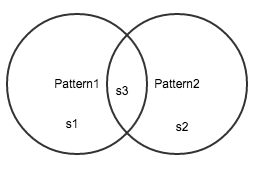
\includegraphics[scale=0.5]{vangraph}    
\end{column}

    
\end{columns}

\end{frame}

\begin{frame}[fragile]
\frametitle{Extended Argument Matching}
\framesubtitle{Analysis on performance}
\textbf{If a pattern has $m$ signature with $k$ dots wildcards.}

The modified NFA/DFA method use $m * (m-k)$ times shape and type checking.   \\
The for-loop based method use $k^{m-k} + k$ times shape and type checking.   \\
\begin{columns}
\begin{column}[T]{0.5\textwidth}
Plot under $m = 10$,                                                         \\
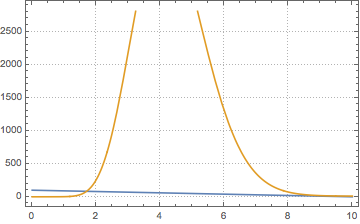
\includegraphics[scale=0.4]{plot}    
\end{column}
\begin{column}[T]{0.5\textwidth}
Plot under $m = 5$,                                                          \\
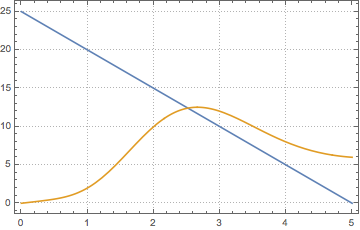
\includegraphics[scale=0.4]{plot_small}    
\end{column}
\end{columns}
$\Rightarrow$                                                                \\
Implemented as for-loop based method for patterns with few dots wildcard
(1-2), NFA/DFA method for other scenario.
\end{frame}

\begin{frame}[fragile]
\frametitle{Extended Argument Matching}
\framesubtitle{Using matcher function}
\textbf{Input argument matching:}
\begin{lstlisting}[basicstyle=\small, language=MATLAB]
foo(var1, var2(:).f, var3{:})
\end{lstlisting} 
$\Rightarrow$
\begin{lstlisting}[basicstyle=\small, language=MATLAB]
AM_VAR_1 = {var1, var2(:), var{:}};
AM_MATCH_RESULT(1) = matcher1(AM_VAR_1);
AM_MATCH_RESULT(2) = matcher2(AM_VAR_2);
% ...
foo(AM_VAR_1{:})
\end{lstlisting}

\textbf{Output argument matching:}
\begin{lstlisting}[basicstyle=\small, language=MATLAB]
foo(var1, var2(:).f, var3{:})
\end{lstlisting} 
$\Rightarrow$
\begin{lstlisting}[basicstyle=\small, language=MATLAB]
% callWithMatcher is a MEX implemented subroutine using C
AM_VAR_1 = {var1, var2(:), var{:}};
[AM_MATCH_RESULT, ...] = callWithMatcher(
                             @foo, AM_VAR_1, 
                             @matcher1, @matcher2, ...
                         );
\end{lstlisting}
\end{frame}

\begin{frame}
\frametitle{Applications and Future Work}
\begin{itemize}
    \item McWeb IDE
    \item Sparse matrix tracing
    \item Type and index checking
    \item ...
\end{itemize}

\pause

\begin{itemize}
    \item Optimizations
    \item OOP features
    \item Static code insertions
    \item ...
\end{itemize}
\end{frame}

\end{document}